

\section{Multicabos}
\label{mulicabos}


\begin{table}[ht!]

	\begin{tabular}{r l|l p{12cm} }
		
		\textcolor{gray}{Especificação} &&& 	{Multicabo 12x24 MPAS 40m}\\
		\textcolor{gray}{Data} &&& 				{28/05/2014}\\
        \textcolor{gray}{Beneficiado} &&&		{RA RA SOM E Acessoria LTDA} \\
        \textcolor{gray}{CNPJ} &&& 				{02.424.555/0001-96} \\
        \textcolor{gray}{Número Nota} &&& 		{476} \\
		\textcolor{gray}{Quantidade} &&& 		{1} \\
		\textcolor{gray}{Valor} &&& 			{R\$494,00} \\
		\textcolor{gray}{Data Sheet} &&& 		{-} \\

		\textcolor{gray}{Função no projeto} &&& {Cabo de 24 vias e 40 metros
		utilizado como umbilical de teste. Terá saída para sensores
		indutivos, sonar, módulo Ethernet, VCC e GND.}
		\\
		\textcolor{gray}{Razão da Escolha} &&& {Cabos para equipamentos de som com
		proteção emborrachada, possui características semelhantes ao ressitente à
		água. O cabo pode ser utilizado para ambiente submarino e é flexível.}
		

	\end{tabular}
\end{table}

\newpage
\subsection{Foto do Material}
\begin{figure}[H]
 \centering
 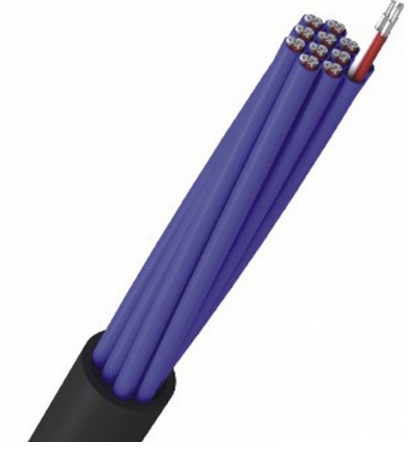
\includegraphics[width=1\columnwidth]{Multicabos/foto.png}
 \caption{Multicabo 24 vias}
\end{figure}

\subsection{Nota Fiscal}
\begin{figure}[H]
 \centering
 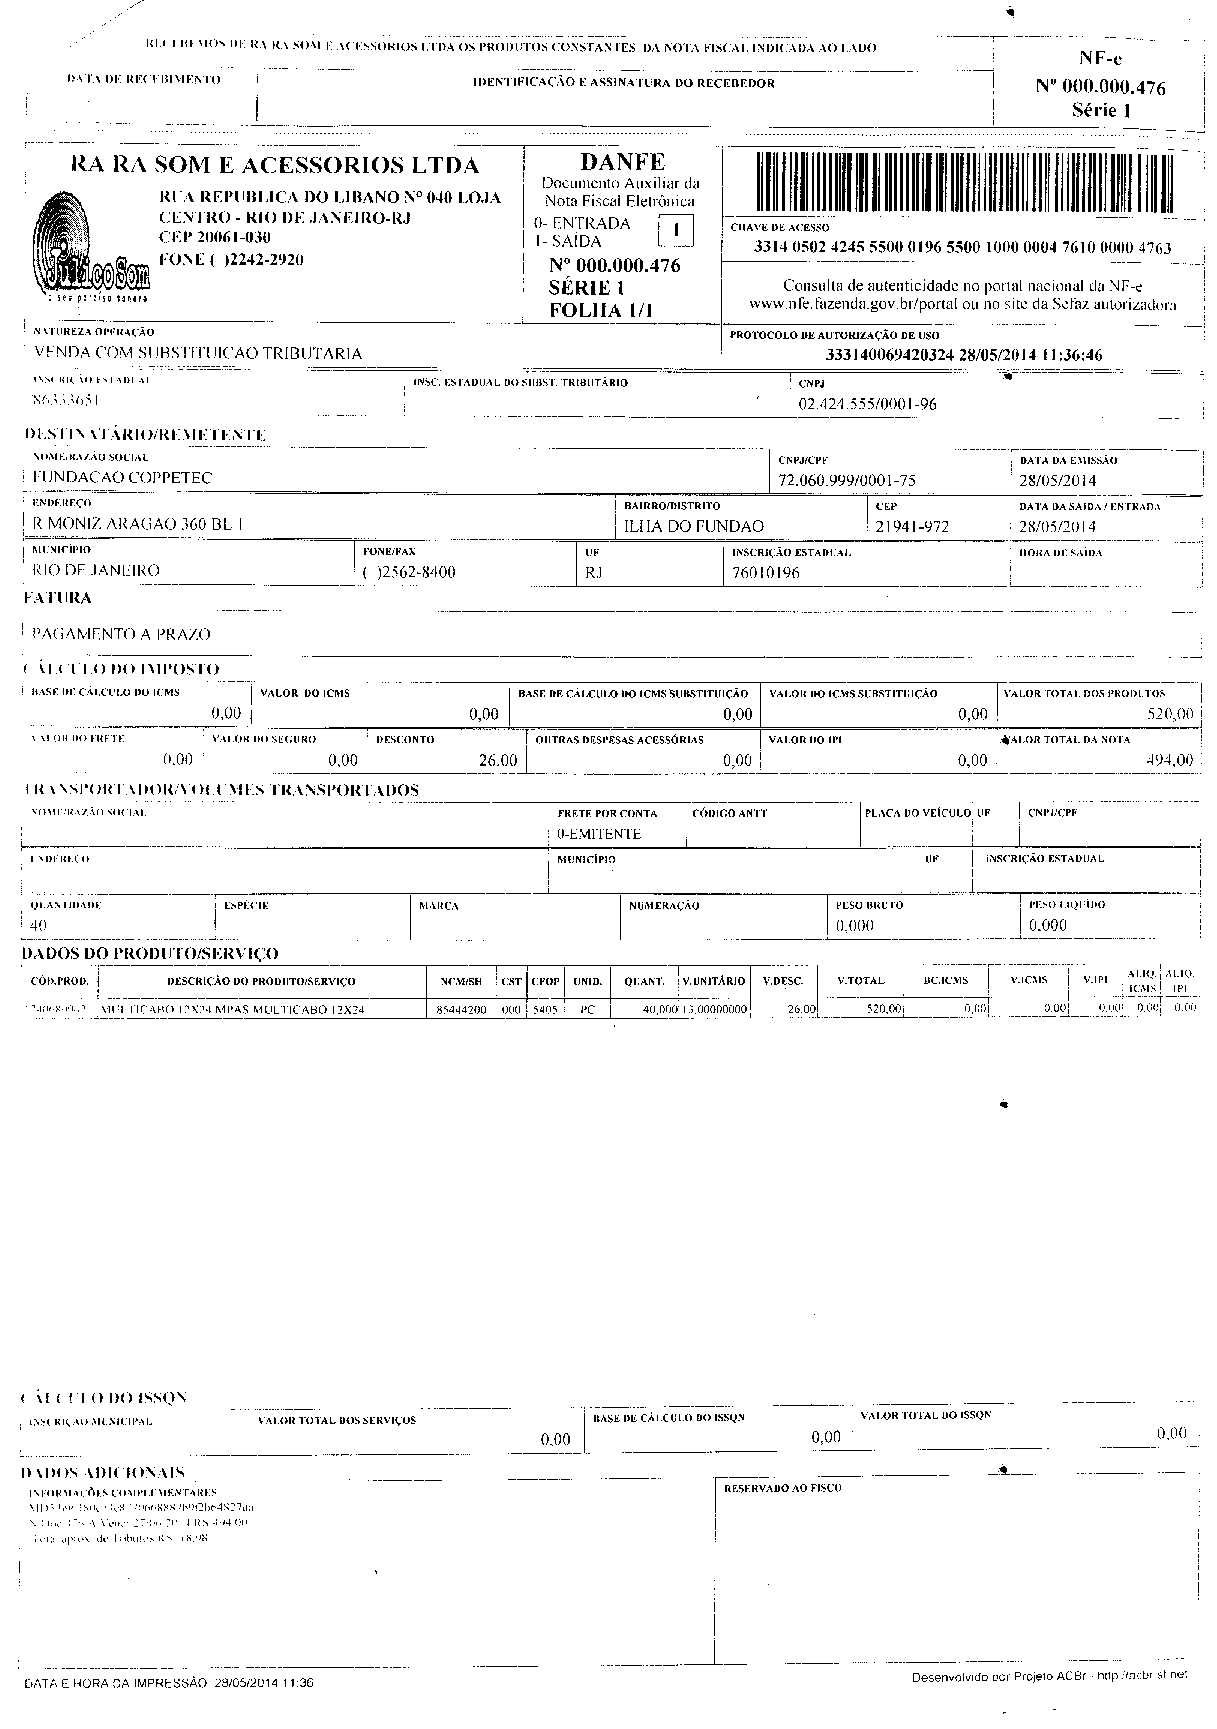
\includegraphics[width=0.9\columnwidth]{Multicabos/nota_multicabos.pdf}
 \caption{Multicabo 24 vias}
 \end{figure}